\chapter{System implementation in Kaldi}
Kaldi is a popular, open-source, speech recognition toolkit that based on weighted finite-state transducers.This chapter is going to describe how Kaldi works to build the AV-ASR system in our music corpus.
\section{Data preparation}

In our asr-music/s5 recipe, some files need to be prepared by hand and get stored in folder asr-music/s5/data, while others can be generated by Kaldi's tools like the table \ref{tab:datafile} below shows.

\begin{table}[ht]
\center
\begin{tabular}{c|c}
files prepared by hand & files generated by Kaldi \\
\hline
utt2spk & spk2utt\\
spk2gender & cmvn.scp\\
text & feats.scp \\
wav.scp &  \\ 
\end{tabular}
\caption{File distribution in prepared data}
\label{tab:datafile}
\end{table}

To know more about what are these data file, here are also some tables to show the format of files prepared by hand.

\begin{table}[ht]
\center
\begin{tabular}{c|c}

utterance-id & speaker-id \\ \hline
F002\_002\_01\_0101.00.001  & F002\_01\\
...\\ \hline
\end{tabular}
\caption{utt2spk format}
\label{tab:utt2spk}
\end{table}

\begin{table}[ht]
\center
\begin{tabular}{c|c}

speaker-id & gender\\ \hline
F002\_01 & f\\
...\\ \hline
\end{tabular}
\caption{spk2gender format}
\label{tab:spk2gender}
\end{table}


\begin{table}[ht]
\center
\begin{tabular}{c|c}

utterance-id & annotation \\ \hline
F002\_002\_01\_0101.00.001  & THIS WAS ALL YOU\\ \hline
...\\ \hline
\end{tabular}
\caption{text format}
\label{tab:text}
\end{table}



\begin{table}[ht]
\center
\begin{tabular}{c|c}

utterance-id & extended-filename \\ \hline
F002\_002\_01\_0101.00.001  & video/mp4\_segments/F/F002/F002\_002\_01\_0101.00.001.mp4\\ \hline
...\\ \hline
\end{tabular}
\caption{wav.scp format}
\label{tab:wav.scp}
\end{table}



\subsubsection{Methods of files generated by Kaldi}
\begin{table}[ht]
\center
\begin{tabular}{ll} \hline
filename & generate tools  \\ \hline
spk2utt & utils/utt2spk\_to\_spk2utt.pl\\ \hline
feats.scp & audio:steps/make\_mfcc.sh \\ \hline
         & video: \\ \hline
         & 1.use extract\_video\_features.py to get utterance-id.lip\_dct.hdf5 \\ \hline
         & 2.convert this hdf5 file into feats.txt with Kaldi's ark format \\ \hline
         & 3.copy-feats ark,t:feats.txt ark,scp:video.ark,feats.scp  \\ \hline
cmvn.scp & steps/compute\_cmvn\_stats.sh\\ \hline
...\\ \hline

\end{tabular}
\end{table}



After get these data prepared, we still need to run utils/validate\_data\_dir.sh to check if anything already prepared well in the data directory. Sometimes it would occur some errors, like 'utt2spk is not in sorted order when sorted first on speaker-id '. Then basically we use utils/fix\_data\_dir.sh to fix it.


\section{Feature extraction}
This section would cover how to extract audio and video features individually and adapt them to be read by Kaldi. 
\subsection{mfcc extraction}
Kaldi’s waveform-reading code can create MFCC and PLP features to do the ASR. 
In our project we choose mfcc as the audio feature, because mel scale can connect the relationship between human’s sensor rate and audio actual frequency. As we know, People is easier to distinguish the slight difference in signal with low frequency, but difficult to sense the variances in signal with high frequency. Besides, as its formula $M(f)=1125\ln (1+\frac{f}{700})$ shows, mel scale focus more on the variances of low frequency signal.
\begin{table}[ht]
\center
\begin{tabular}{c|c}
frequency  & Mel frequency\\ \hline
300 Hz  & 401.25 mels\\ 
1000 Hz  & 997.87 mels\\
8000 Hz  & 2834.99 mels\\ 
...\\ \hline
\end{tabular}
\caption{transform between f with Mel(f)}
\label{tab:melf}
\end{table}

From the table \ref{tab:melf}, we can see Mel frequency narrow the scope of frequency, but mostly effect on the original frequency that higher than 1000Hz.  In this way, Mel scale put a large weight on low frequency signal and a small weight on high frequency signal.  It is a similar process comparing with the work of human’s hearing.  Therefore, mfcc is more suitable to be the audio feature in this ASR system for song transcription.
And after extracting the mfcc feature, it is good to do Cepstral Mean Normalisation on them to balance the average feature value.

\section{Video feature extraction}

To develop the visual front end of ASR, video feature extraction is an important step. For Kaldi doesn’t provide methods for video feature, we have to extract video features individually and convert them into kaldi format in order to be read.

This process aims to extract sequences of 2D-dct transformed lip region frames of utterances. To achieve that, there are mainly 4 steps. 
\begin{enumerate}
\item  Detect the face in the frames and locate them as landmarks

Here we use open-source dlib toolkit, which is implemented with the ensemble regression tree method (Kazemi and Sullivan, 2014) to extract histogram of oriented gradients feature in order to detect 68 landmarks feature. As the picture \ref{img:face68} shows, this is an example for dlib toolkit to detect face landmarks whose speaker id is M020 in our database.

\begin{center}
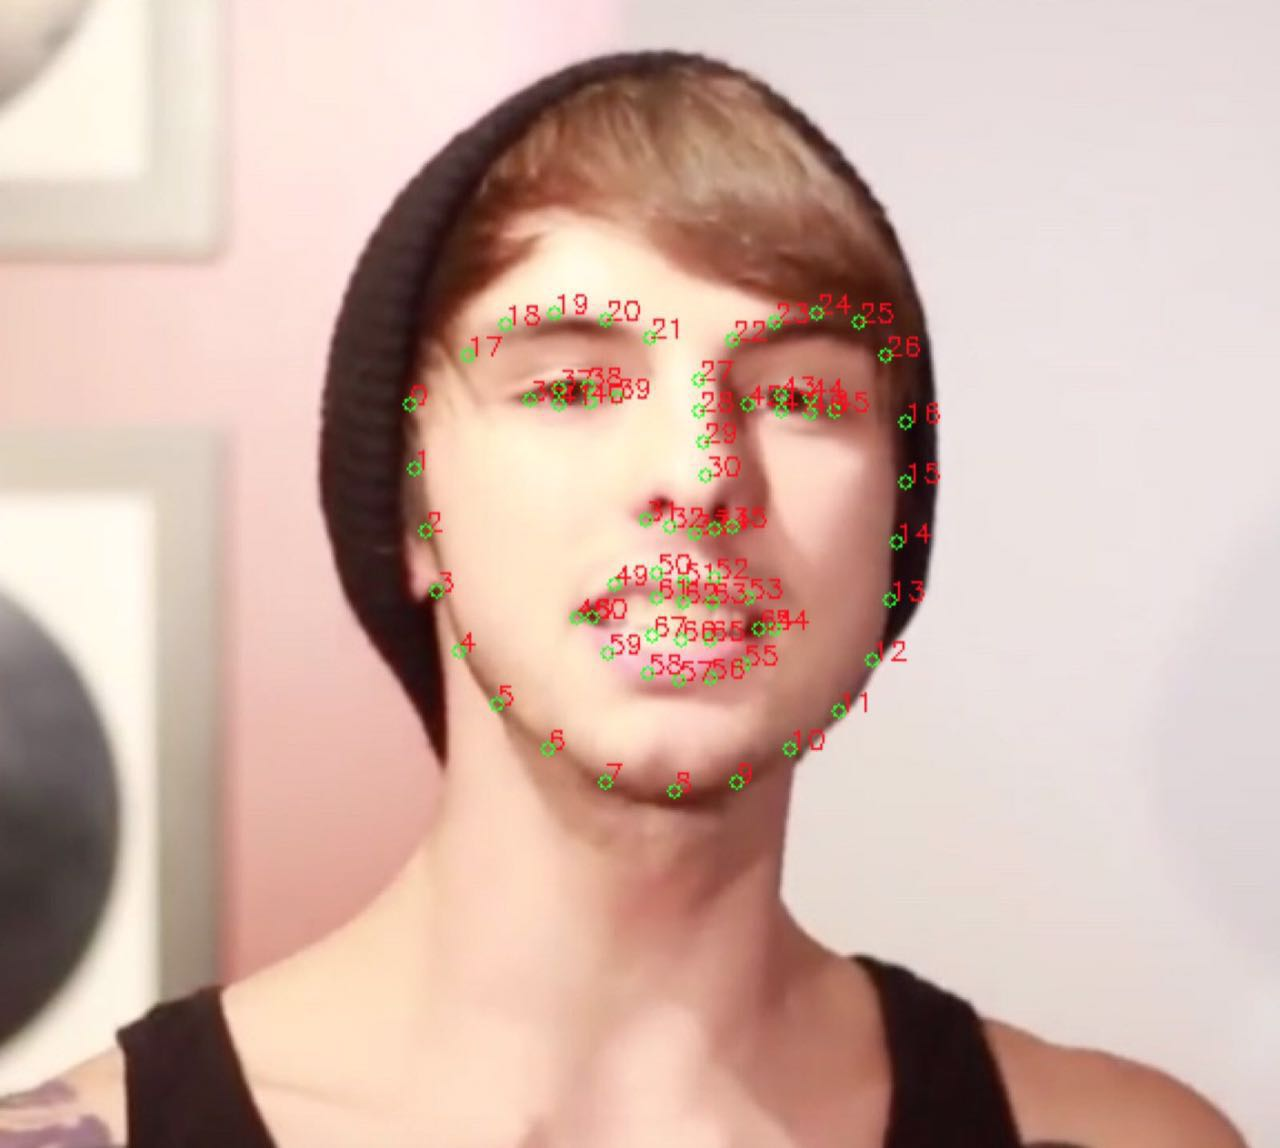
\includegraphics[width=0.5\linewidth]{images/face68.jpg}
\label{img:face68}
\end{center}
\item Adapt the affine transform into frames

Speaker in this picture has a frontal face to the camera, but it still has many faces can be detected with 68 landmarks but they only have side-face to the camera. Therefore, the affine transform is needed to normalize the impact of different head poses. In order to perform the affine transform, we set a landmark template, which is calculated by average frontal face landmarks in AV Lombard Grid corpus[6]. And then we compute the transform with RANSAC fitting algorithm.
\item Extract the ROI

The ROI is a fix-sized bounding box based on the coordinates of outer lip landmarks. Because the height and width are set by 1.2 multiply (max(x)-min(x)) and (max(y)-min(y)) of  these lip landmarks. Even though the size of bounding box is fixed, they’re only fixed in the same utterance of video. Therefore, we can extract the ROI and they are in RGB pixels.

\item Perform a 2d-dct on the ROI pixels to compress the frames information and remove correlation.

Before this, it is also necessary to rescale ROI on each frame to a fixed size of 240 by 240 and convert RGB vectors into YUV color space. Finally, we set the number of max feature count as 55, and then do the diagonal scanning on DCT matrix in order to achieve the 2 dimensional dct feature with 55 elements.

\end{enumerate}

\subsection{Video feature fusion with kaldi format}

To convert video feature into Kaldi’s format, we need to know what format the feature data present in the Kaldi. Kaldi has its script called make\_mfcc.sh can generate the mfcc feature and we can check the format with Kaldi’s binary file called copy-feats. Here is the mfcc feature and cmvn\_mfcc feature of the former 2 frames in utterance F002\_002\_01\_0101.00.001, as we can see, every frame has 13 vectors.
\begin{center}
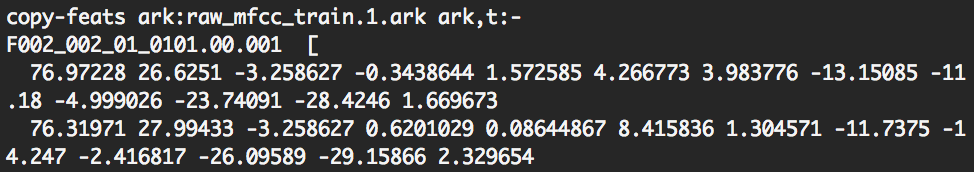
\includegraphics[width=1\linewidth]{images/train_mfcc.png}\\
\label{img:mfcc}
\end{center}
The cmvn\_mfcc feature is generated by running the script in kaldi called compute\_cmvn\_stats.sh in order to make mfcc features robust to some linear filtering of the signal. 
\begin{center}
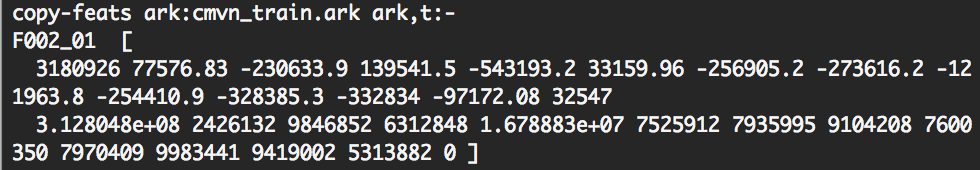
\includegraphics[width=1\linewidth]{images/cmvn_mfcc.png}\\
\label{img:cmvnmfcc}
\end{center}
The next step is to transfer video feature’s vectors with mfcc Kaldi’s format. The images below show the video feature vectors of the same utterance 
F002\_002\_01\_0101.00.001.
\begin{center}
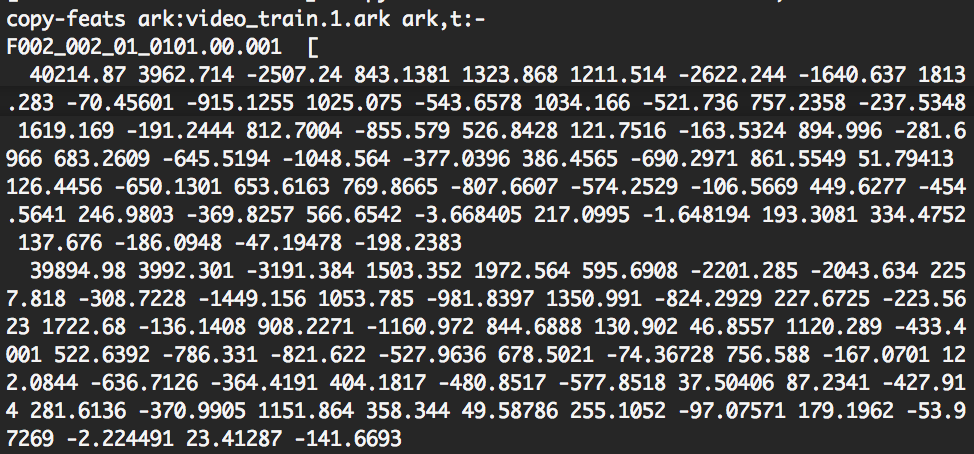
\includegraphics[width=1\linewidth]{images/train_video.png}\\
\label{img:video}
\end{center}

\begin{center}
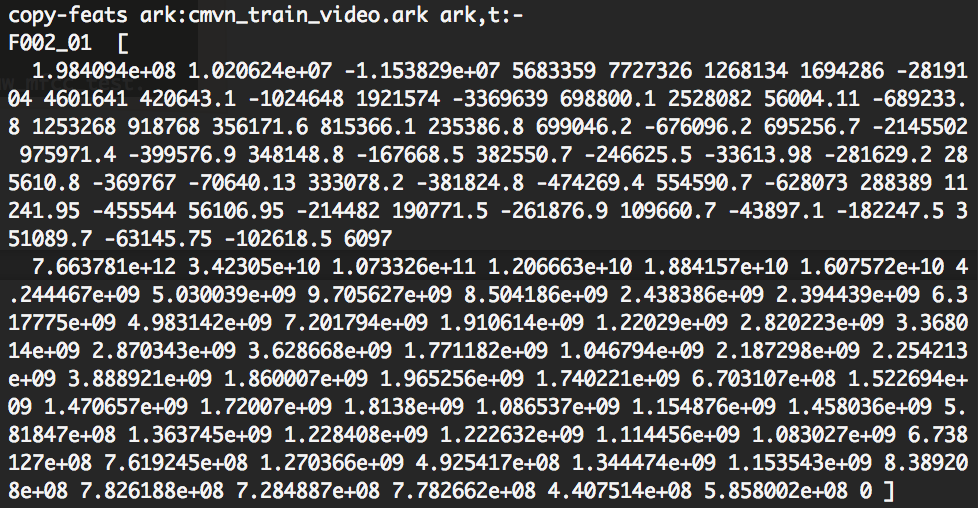
\includegraphics[width=1\linewidth]{images/cmvn_video.png}\\
\label{img:cmvnvideo}
\end{center}

\subsection{Generate Language model}
Since Kaldi is based on WFST framework, it provide tools to make standard arpa format represented as fst. In our recipes, we need to install and build the IRSTLM toolkit and use that to build language models from raw text.
In our project, we would generate uni-gram, bi-gram and tri-gram language model, and use them respectively to decode different acoustic models.
\subsection{ Train Acoustic models }
Training acoustic models with HMM-GMM method is a process of updating the parameters of HMM and GMM. In this project, we would use a few of Kaldi's scripts like train\_mono.sh, train\_deltas.sh, and train\_lda\_mllt.sh to train the acoustic models.
And the detailed steps of training acoustic models can be stated as follows:
\begin{enumerate}
\item Initialize GMM and output o.ml and tree file.
\item Compile training graphs and output fits.JOB.gz with o.mdl, tree and L.fst as input files.
\item Align the text annotation with frames with bin/align-equal-compiled binary file.
\item Do Maximum likelihood estimate on states which are based on GMM with gmmbin/gmm-est and get the parameter of GMM.
\item Iterate the process.
\item Accumulate the states based on GMM and do Maximum likelihood estimate  again to get the most likely sequence of states.
\item Merge the Maximum likelihood estimate results and generate the .mdl file.
\item Increase the number of guassians. If not surpass the number of iteration, return to the step 5 to train again.
\item Generate the final.mdl file as system's acoustic model.
\end{enumerate}

\subsection{Decode}
In this section, we need decode the training data with a suitable language model matching the trained acoustic model and then create the decoding graphs. For G.fst is a presentation of language model, L.fst is a presentation of lexicon dictionary, C.fst represents the context-dependent information and H.fst represents HMM, the process of decoding is to build a Transducer from the substate of context-dependent phoneme to word with viterbi algorithm.

\subsection{Evaluation methodology}

The most common way of evaluating an ASR system is to calculate the WER. To the specific AV-ASR system in music, there are also some specific methods to evaluate the system’s performance. For example, considering of the characteristics of different instrument, the effect degree to singing voice should be different as well. Therefore, we can separate songs by the type of accompanied-instrument and group them into different folders to exploit the effect of different instrument. Similar methods like pitch, tempo modification with dataset, also can be effect the audio-only ASR system's performance. For videos, we also can group songs into different folders according to the quality of video frames. Sometimes, the Lip region is partly sheltered from microphone or the frame has no face to be detected, any of them can reduce the performance of results. 

On the other hand, not in terms of modifying the input data. We can update the system's WER by adjusting the phone type of acoustic model and the size of n-gram language models. 





